\documentclass[UTF8]{article} % chinese
\usepackage{ctex}
%\documentclass{article}     %english
%\usepackage[nonatbib]{neurips}
\usepackage[final]{aneurips}
\usepackage[utf8]{inputenc} % allow utf-8 input
\usepackage[T1]{fontenc}    % use 8-bit T1 fonts
\usepackage{hyperref}       % hyperlinks
\usepackage{url}            % simple URL typesetting
\usepackage{booktabs}       % professional-quality tables
\usepackage{amsfonts}       % blackboard math symbols
\usepackage{nicefrac}       % compact symbols for 1/2, etc.
\usepackage{microtype}      % microtypography
\usepackage{amsmath}
\usepackage{bm}
\usepackage{float}
\usepackage{enumitem}
\usepackage{multirow}
\usepackage{adjustbox}
\usepackage{color,xcolor,colortbl}
\usepackage[ruled, vlined, linesnumbered]{algorithm2e}
\newcommand{\mycomment}{\color{black}}
\newtheorem{lemma}{Lemma}
\newtheorem{theorem}{Theorem}
\graphicspath{{figure/}{images}}


\title{Paper Title}

\author{%
  Author First\thanks{corresponding author} \\
  Department of Computer \\
  Beijing University of Chemical Technology \\
  \texttt{first@mail.buct.edu.cn} \\
  \And
  Author Second \\  
  Department of Computer \\
  Beijing University of Chemical Technology \\
  \texttt{second@mail.buct.edu.cn} \\
}

\begin{document}

\maketitle

\begin{abstract}
Graph Neural Networks (GNN) is an emerging field for learning on non-Euclidean data. Recently, there has been great interest in designing GNN that scales to large graphs. Most existing techniques use ``graph sampling'' or ``layer-wise sampling'' technique to reduce training time. 

解决了什么问题?论文主要工作?效果如何?
~\\
~\\
~\\
\end{abstract}

\section{Introduction}
Recently, the field of Graph Neural Network has drawn increasing attention due to its wide range of applications such  as social analysis, biology, recommendation system, and computer vision. Graph Neural Network (GCN) adopts a message-passing approach and gathers information from the neighbors of each node from the previous layer to form new representation. The vanilla GCN uses a full-batch training process and stores each node's representation in the GPU memory, which leads to limited scalability. On the other hand, training GCN with mini-batches is difficult, as the neighborhood size could grow exponentially with the number of layers.

论文所处的背景
~\\
~\\
~\\


当前的现状?
~\\
~\\
~\\

本文所做的主要工作和贡献
~\\
~\\
~\\

\paragraph{Our contribution.} In this paper, we first carefully analyze the theoretical complexity of existing scalable GNNs and explain why they cannot scale to graphs with billions of edges. Then, we present GBP (Graph neural network via Bidirectional Propagation), a scalable Graph Neural Network with sub-linear time complexity in theory and superior performance in practice. 

~\\
~\\
~\\

\section{Related work}
\subsection{Work1}

~\\
~\\
~\\

\subsection{Work2}

~\\
~\\
~\\

\subsection{Work3}

~\\
~\\
~\\

\section{Proposed Method}

这里是论文最重要的部分,描述自己的方法。
~\\
~\\
~\\

\subsection{Analysis}\label{sec:analysis}
~\\
~\\
~\\


\section{Experiments}
\paragraph{Datasets} 

\begin{table}[ht]
\vspace{-4mm}
\begin{center}\small
\caption{Dataset statistics.}
\label{dataset-table}
\begin{tabular}{llrrrrr}
\toprule
Dataset & Task & Nodes & Edges & Features & Classes &  Label rate \\
\midrule
Cora & multi-class & 2,708 & 5,429      & 1,433         & 7 & 0.052            \\
Citeseer    & multi-class& 3,327       & 4,732       & 3,703   & 6 & 0.036     \\
Pubmed      & multi-class& 19,717      & 44,338      & 500       & 3  & 0.003  \\
PPI         & multi-label& 56,944      & 818,716     & 50    & 121 & 0.79      \\
Yelp        & multi-label& 716,847     & 6,977,410   & 300  & 100 & 0.75       \\
Amazon      & multi-class& 2,449,029   & 61,859,140  & 100  & 47 & 0.70        \\
Friendster  & multi-class& 65,608,366 & 1,806,067,135 & 100 (random) & 500 & 0.001  \\
\bottomrule    
\end{tabular}
\end{center}
%\vspace{-0.35cm}
\vspace{-4mm}
\end{table}

\paragraph{Baselines and detailed setup}
~\\
~\\
~\\

\begin{table}[ht]
\begin{center}
\caption{Results on Cora, Citeseer and Pubmed.}
\label{transductive-table}
\begin{tabular}{llll}
\toprule
Method & Cora & Citeseer & Pubmed \\
\midrule
GCN & 81.5 $\pm$ 0.6 & 71.3 $\pm$ 0.4 & 79.1 $\pm$ 0.4 \\
GAT & 83.3 $\pm$ 0.8& 71.9 $\pm$ 0.7 & 78.0 $\pm$ 0.4\\
GDC & 83.3 $\pm$ 0.2 & 72.2 $\pm$ 0.3 & 78.6 $\pm$ 0.4 \\
APPNP & 83.3 $\pm$ 0.3 & 71.4 $\pm$ 0.6 & 80.1 $\pm$ 0.2 \\
SGC    & 81.0 $\pm$ 0.1 & 71.8 $\pm$ 0.1 & 79.0 $\pm$ 0.1 \\
LADIES& 79.6 $\pm$ 0.5 & 68.6 $\pm$ 0.3 & 77.0 $\pm$ 0.5 \\
PPRGo & 82.4 $\pm$ 0.2 & 71.3 $\pm$ 0.3 & 80.0 $\pm$ 0.4 \\
GraphSAINT& 81.3 $\pm$ 0.4 & 70.5 $\pm$ 0.4 & 78.2 $\pm$ 0.8 \\
\midrule
GBP  & \textbf{83.9 $\pm$ 0.7} & \textbf{72.9 $\pm$ 0.5} & \textbf{80.6 $\pm$ 0.4} \\
\bottomrule
\end{tabular}
\end{center}
\vspace{-0.35cm}
\end{table}

\paragraph{Inductive learning on medium to large graphs}
~\\
~\\
~\\

\begin{figure}[ht]
\begin{center}
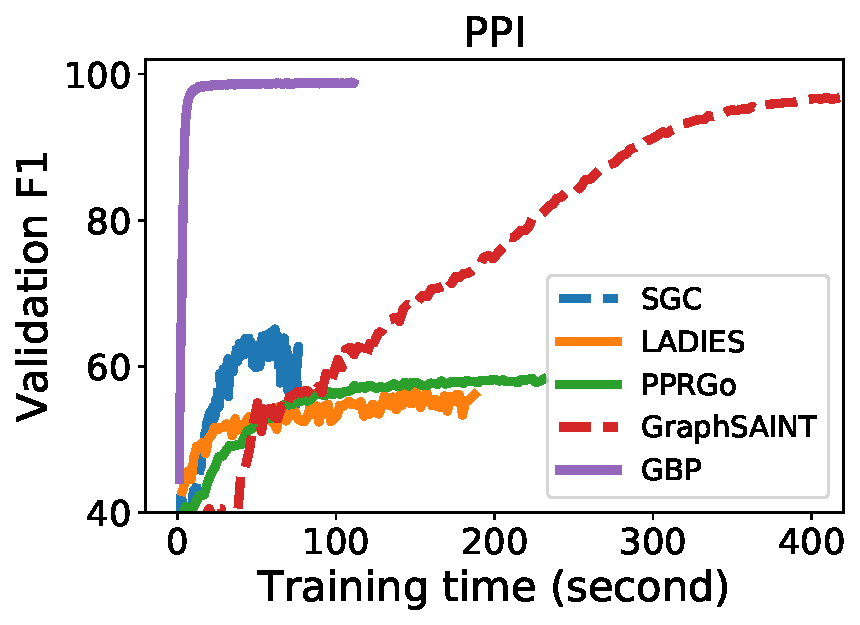
\includegraphics[height=33mm]{ppi.pdf}
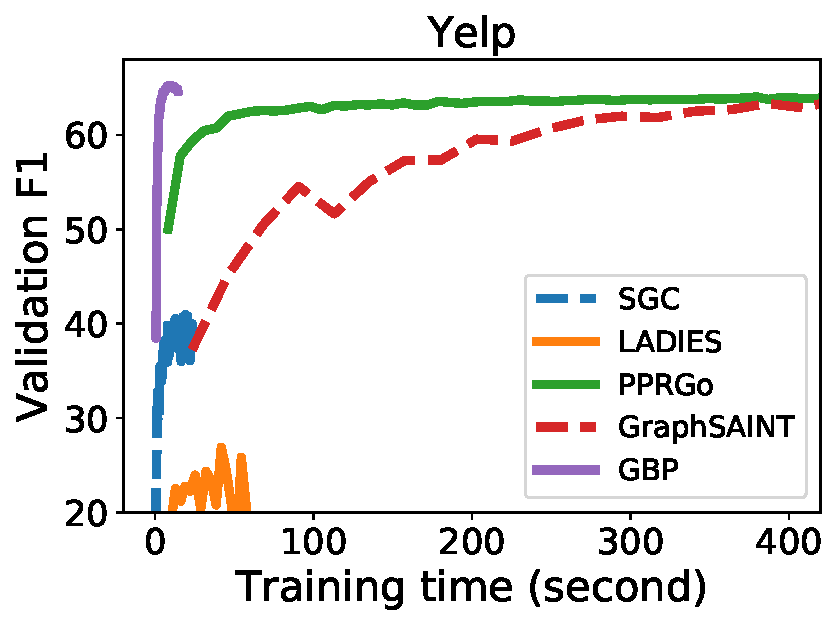
\includegraphics[height=33mm]{yelp.pdf}
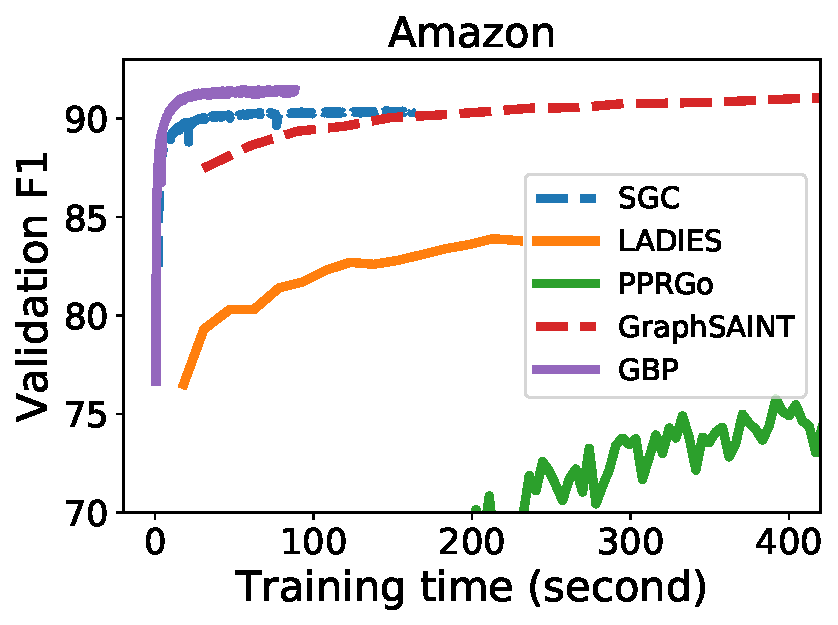
\includegraphics[height=33mm]{amazon.pdf}
\vspace{-2mm}
\caption{Convergence curves of 4-layer models.} 
\vspace{-2mm}
\label{fig:convergence}
\end{center}
\vspace{-0.35cm}
\end{figure}

\paragraph{Transductive semi-supervised learning on billion-scale graph Friendster.}
~\\
~\\
~\\

\section{Conclusion}
~\\
~\\
~\\

\section*{Acknowledgments}
~\\
~\\
~\\

\bibliographystyle{abbrv}
\bibliography{E:/studio/learn/python/src/bench/bibtex/complete.bib}
\end{document}
